\subsection{Directed Acyclic Graphs in Spark}
Con tutti i vari job, Spark crea un flusso logico di operazioni, che è noto come \textbf{Directed Acyclic Graph (DAG)}. In Spark, un DAG è un grafo diretto aciclico dove i \textit{vertici} rappresentano le strutture dati (RDD o DataFrame) e gli \textit{archi} rappresentano l'operazione da applicare su di esse. Alla chiamata di un'azione, il DAG creato viene sottoposto al \textit{DAGScheduler} che divide ulteriormente il grafo nelle fasi da svolgere per portare a termine il compito. Questo aiuta a: ridurre al minimo il rimescolamento dei dati, ridurre la durata dei calcoli, migliorare l'efficienza del processo nel tempo.

Inoltre, Spark sfrutta la strategia denominata \textbf{lazy evaluation}, ovvero posticipa la valutazione di un'espressione finché non è necessaria. Per le trasformazioni, Spark le aggiunge a un DAG e solo quando il driver richiede alcuni dati, questo DAG viene effettivamente eseguito. Ciò significa che, memorizzando ogni dettaglio delle operazioni eseguite su diverse partizioni di RDD, è possibile recuperare facilmente dati persi in caso di fallimento o di perdita di qualsiasi RDD.
\begin{figure}[hbt!]
    \centering
    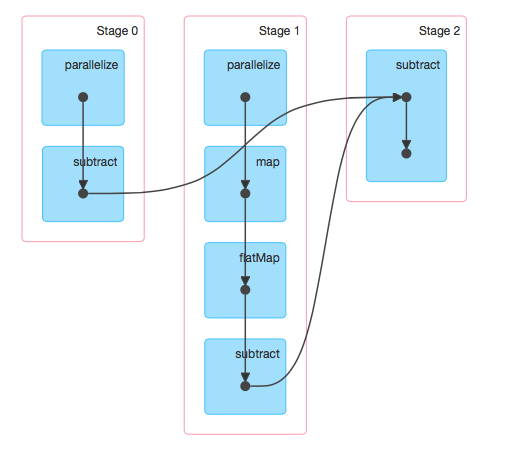
\includegraphics[width=0.8\textwidth]{img/sparkdag.png}
    \caption{Esempio di Spark DAG}
    \label{fig:spark_dag}
\end{figure}

